%
%!TEX root = ../../../hp3D_user_guide.tex
%

%--------------------------------------------------------------------

\section{Poisson Problems}
\label{sec:poisson}

For the first model problem implementation, we consider the Poisson problem with inhomogeneous Dirichlet BC:
\begin{alignat*}{3}
	- \div \nabla u &= f && \quad \text{in } \Omega \, , \\
	u &= u_0 && \quad \text{on } \Gamma \, .
\end{alignat*}

Classical variational formulation:
\[
\left\{
\begin{array}{llll}
	u \in H^1(\Omega):  u = u_0 \text{ on } \Gamma \, , \\[5pt]
	(\nabla u, \nabla v) = (f,v) \, ,
	\quad v \in H^1(\Omega) \, : \, v = 0 \text{ on } \Gamma \, .
\end{array}
\right.
\]

\subsection{Galerkin implementation}
\label{subsec:poisson-galerkin}

The Galerkin FE implementation of the variational problem is located in the application directory \file{problems/POISSON/GALERKIN}. In the remainder of this section, file paths may be given as relative paths within the application directory.

Input files:
\begin{itemize}
	\item{\file{control/control}: sets global control variables, e.g.
	\begin{itemize}
		\item \var{NEXACT} $\in \{$ \code{0,1} $\}$: indicates whether the exact solution is known.
		\item \var{EXGEOM} $\in \{$ \code{0,1} $\}$: indicates whether isoparametric or exact-geometry elements are used.
	\end{itemize}
	}
	\item{\file{input/physics}: sets initially allocated nodes and physics variables.
\begin{lstlisting}[caption=\file{POISSON/GALERKIN/input/physics} input file.]
100000              MAXNODS, nodes anticipated
1                   NR_PHYSA, physics attributes
field   contin  1   H1 variable
\end{lstlisting}
	\begin{itemize}
		\item The value of \var{MAXNODS} does not have to be precise; if more nodes are needed, the code allocates them on-the-fly. However, it is recommended for efficiency that the code does not reallocate, as well as not selecting \var{MAXNODS} much larger than needed.
		\item \code{\var{NR\_PHYSA}=1} specifies that \emph{one} physics variable is declared.
		\item \code{`field   contin  1'} specifies ``nickname, approximation space, number of components'' of a variable. The approximation spaces are: $H^1$ -- \code{contin}, $H(\tcurl)$ -- \code{tangen}, $H(\tdiv)$ -- \code{normal}, $L^2$ -- \code{discon}.
		\item For this Galerkin FE formulation, one $H^1$ variable is needed.
	\end{itemize}
	}
	\item{\file{geometries/hexa\_orient0}: defines the initial geometry mesh (a cube).}
\end{itemize}

Next, we take a look at the required routines that must be provided by the user:
\begin{itemize}
	\itemsep 0pt
	\item
	{\routine{set\_initial\_mesh}:\\
	for \emph{each} initial mesh element, this routine sets
	\begin{itemize}
		\itemsep 0pt
		\item the supported physics variables;
		\item the initial polynomial order of approximation;
		\item the boundary condition flags for element faces on the boundary.
	\end{itemize}
\begin{lstlisting}[caption=\file{POISSON/GALERKIN/}\routine{set\_initial\_mesh} routine.]
!..loop over initial mesh elements
   do iel=1,NRELIS

!  ...1. set physics
      ELEMS(iel)%nrphysics = 1
      allocate(ELEMS(iel)%physics(1))
      ELEMS(iel)%physics(1) ='field'

!  ...2. set initial order of approximation
      select case(ELEMS(iel)%etype)
         case(TETR); Nelem_order(iel) = 1*IP
         case(PYRA); Nelem_order(iel) = 1*IP
         case(PRIS); Nelem_order(iel) = 11*IP
         case(BRIC); Nelem_order(iel) = 111*IP
      end select

!  ...3. set BC flags: 0 - no BC ; 1 - Dirichlet; 2-9 Custom BCs
      ibc(1:6,1) = 0
      do ifc=1,nface(ELEMS(iel)%etype) ! loop through element faces
         neig = ELEMS(iel)%neig(ifc)
         select case(neig)
            case(0); ibc(ifc,1) = 1
         end select
      enddo

!  ...allocate BC flags (one per component), 
!     and encode face BCs into a single BC flag
      allocate(ELEMS(iel)%bcond(1))
      call encodg(ibc(1:6,1),10,6, ELEMS(iel)%bcond(1))
   enddo
\end{lstlisting}
	}
	\item
	{\routine{dirichlet}:
	\begin{itemize}
	\item User-provided routine required by the system routine \routine{update\_Ddof} which computes the Dirichlet DOFs for element nodes (vertices, edges, faces) with a non-homogeneous Dirichlet BCs. 
	\item \routine{update\_Ddof} interpolates $H^1$, $H(\tcurl)$, $H(\tdiv)$ Dirichlet data using \emph{projection-based} interpolation.\footnote{\fullcite{demkowicz2008interp}}
	\item Required only if non-homogeneous Dirichlet BCs were set by the user in \routine{set\_initial\_mesh}.
\end{itemize}

\begin{lstlisting}[caption=\file{POISSON/GALERKIN/common/}\routine{dirichlet} routine.]
!  routine dirichlet: returns Dirichlet data at a point
!   in:   Mdle          - middle node number
!         X             - a point in physical space
!         Icase         - node case (specifies supported variables)
!   out:  ValH, DvalH   - value of the H1 solution, 1st derivatives
!         ValE, DvalE   - value of the H(curl) solution, 1st derivatives
!         ValV, DvalV   - value of the H(div) solution, 1st derivatives
subroutine dirichlet(Mdle,X,Icase, ValH,DvalH,ValE,DvalE,ValV,DvalV)
\end{lstlisting}
	}
	\item
	{\routine{elem}:
	\begin{itemize}
	\item User-provided routine that computes the element-local stiffness matrix and load vector.
	\item System module \module{assembly} provides global arrays for this purpose:
	\begin{itemize}
		\item \var{ALOC(:,:)\%array}: Element-local stiffness matrix.
		\item \var{BLOC(:)\%array}: Element-local load vector.
		\item These arrays are declared \omp{omp threadprivate} for shared-memory parallel assembly of different element matrices with OpenMP threading.
	\end{itemize}
\end{itemize}

\routine{elem} is called during assembly for each middle node \var{Mdle} in the \emph{active mesh}.

\begin{remark}
Constrained approximation, modification for Dirichlet nodes, and static condensation of element-interior (bubble) DOFs are automatically done afterwards by the system routine \routine{celem\_system} which provides the \emph{modified element} matrices to the assembly procedure.
\end{remark}

\begin{lstlisting}[mathescape,caption=\file{POISSON/GALERKIN/}\routine{elem} routine]
!..determine element type; number of vertices, edges, and faces
   etype = NODES(Mdle)%ntype
   nrv = nvert(etype); nre = nedge(etype); nrf = nface(etype)
   
!..determine order of approximation
   call find_order(Mdle, norder)
   
!..determine edge and face orientations
   call find_orient(Mdle, norient_edge,norient_face)
   
!..determine nodes coordinates
   call nodcor(Mdle, xnod)
   
!..set quadrature points and weights
   call set_3D_int(etype,norder,norient_face, nrint,xiloc,waloc)

!  ....... element integrals:

!..loop over integration points
   do l=1,nrint

!  ...coordinates and weight of this integration point
      xi(1:3) = xiloc(1:3,l); wa = waloc(l)

!  ...H1 shape functions (for geometry)
      call shape3DH(etype,xi,norder,norient_edge,norient_face, nrdofH,shapH,gradH)

!  ...geometry map
      call geom3D(Mdle,xi,xnod,shapH,gradH,nrdofH, x,dxdxi,dxidx,rjac,iflag)

!  ...integration weight
      weight = rjac*wa

!  ...get the RHS
      call getf(Mdle,x, fval)

!  ...loop through H1 test functions
      do k1=1,nrdofH

!     ...Piola transformation: $q \rightarrow \hat q$ and $\nabla q \rightarrow J^{-T} \hat \nabla \hat q$
         q = shapH(k1)
         dq(1:3) = gradH(1,k1)*dxidx(1,1:3) + &
                    gradH(2,k1)*dxidx(2,1:3) + &
                    gradH(3,k1)*dxidx(3,1:3)

!     ...accumulate for the load vector: $(f,q)$
         b_loc(k1) = b_loc(k1) + q*fval*weight

!     ...loop through H1 trial functions
         do k2=1,nrdofH

!        ...Piola transformation: $p \rightarrow \hat p$ and $\nabla p \rightarrow J^{-T} \hat \nabla \hat p$
            p = shapH(k2)
            dp(1:3) = gradH(1,k2)*dxidx(1,1:3) + &
                       gradH(2,k2)*dxidx(2,1:3) + &
                       gradH(3,k2)*dxidx(3,1:3)

!        ...accumulate for the stiffness matrix: $(\nabla p, \nabla q)$
            a_loc(k1,k2) = a_loc(k1,k2) + weight*(dq(1)*dp(1)+dq(2)*dp(2)+dq(3)*dp(3))

   enddo; enddo; enddo
\end{lstlisting}
	}
\end{itemize}

This concludes the list of necessary input files and routines required for defining the application code from the library-perspective. However, the user is encouraged to take a look at the remaining files within the \file{POISSON/GALERKIN} directory which include the driver \routine{main} and a variety of auxiliary files. In a future version of the user manual, we may include a discussion of these auxiliary files as well.

\subsection{DPG primal implementation}
\label{sec:poisson-primal}

Broken primal DPG formulation:
\[
\left\{
\begin{array}{llll}
	(u, \hat \sigma_n) \in H^1(\Omega) \times H^{-1/2}(\Gamma_h): u = u_0 \text{ on } \Gamma \, , \\[5pt]
	(\nabla u, \nabla v) - \lb \hat \sigma_n , v \rb_{\Gamma_h} 
	= (f,v) \, ,\quad v \in H^1(\Omega_h) \, .
\end{array}
\right.
\]

Compared to the Galerkin FE implementation, the primal DPG implementation mostly differs in the \routine{elem} routine. In practice, the DPG method is implemented in its mixed form \cite{demkowicz2017dpg} but the extra unknown---the Riesz representation of the residual---is statically condensed on the element level (see Appendix~\ref{chap:dpg}).

The implementation is provided in \file{problems/POISSON/PRIMAL\_DPG}.

Compared to the input files for the Galerkin implementation, the only change is in the \file{physics} file:
\begin{lstlisting}[caption=\file{POISSON/PRIMAL\_DPG/input/physics} input file.]
100000              MAXNODS, nodes anticipated
2                   NR_PHYSA, physics attributes
field   contin  1   H1 variable
trace   normal  1   H(div) variable
\end{lstlisting}
We now have specified two physics unknowns---$u$ and $\hat \sigma_n$, i.e.~\code{\var{NR\_PHYSA}=2}. The additional trace unknown $\hat \sigma_n$ is declared as an $H(\tdiv)$ variable in the \file{physics} file; the normal trace $\hat \sigma_n$ must later be specified as such by setting \code{\var{PHYSAi(2)}=.true.} (e.g.~in the \routine{main} driver).

The \routine{elem} routine for DPG formulations can be structured into three distinct steps:
\vskip 5pt

\begin{minipage}{0.48\textwidth}
\begin{enumerate}
	\itemsep -10pt
	\item Element integration \vspace{-15pt}
	\begin{itemize}
		\itemsep -8pt
		\item Stiffness: $\mr B$
		\item Load: $\mr l$
		\item Gram matrix: $\mr G$
	\end{itemize}
	\item Boundary integration \vspace{-15pt}
	\begin{itemize}
		\itemsep -8pt
		\item Stiffness: $\mr{\hat B}$
	\end{itemize}
	\item Constructing DPG linear system \vspace{-15pt}
	\begin{itemize}
		\itemsep -8pt
		\item Dense linear algebra
		\item {Statically condensed system\\[-5pt] 
		stored in \var{ALOC}, \var{BLOC}}
	\end{itemize}
\end{enumerate}
\end{minipage}%
\begin{minipage}{0.48\textwidth}
\begin{figure}[H]
	\centering
	\begin{subfigure}[b]{0.6\textwidth}
		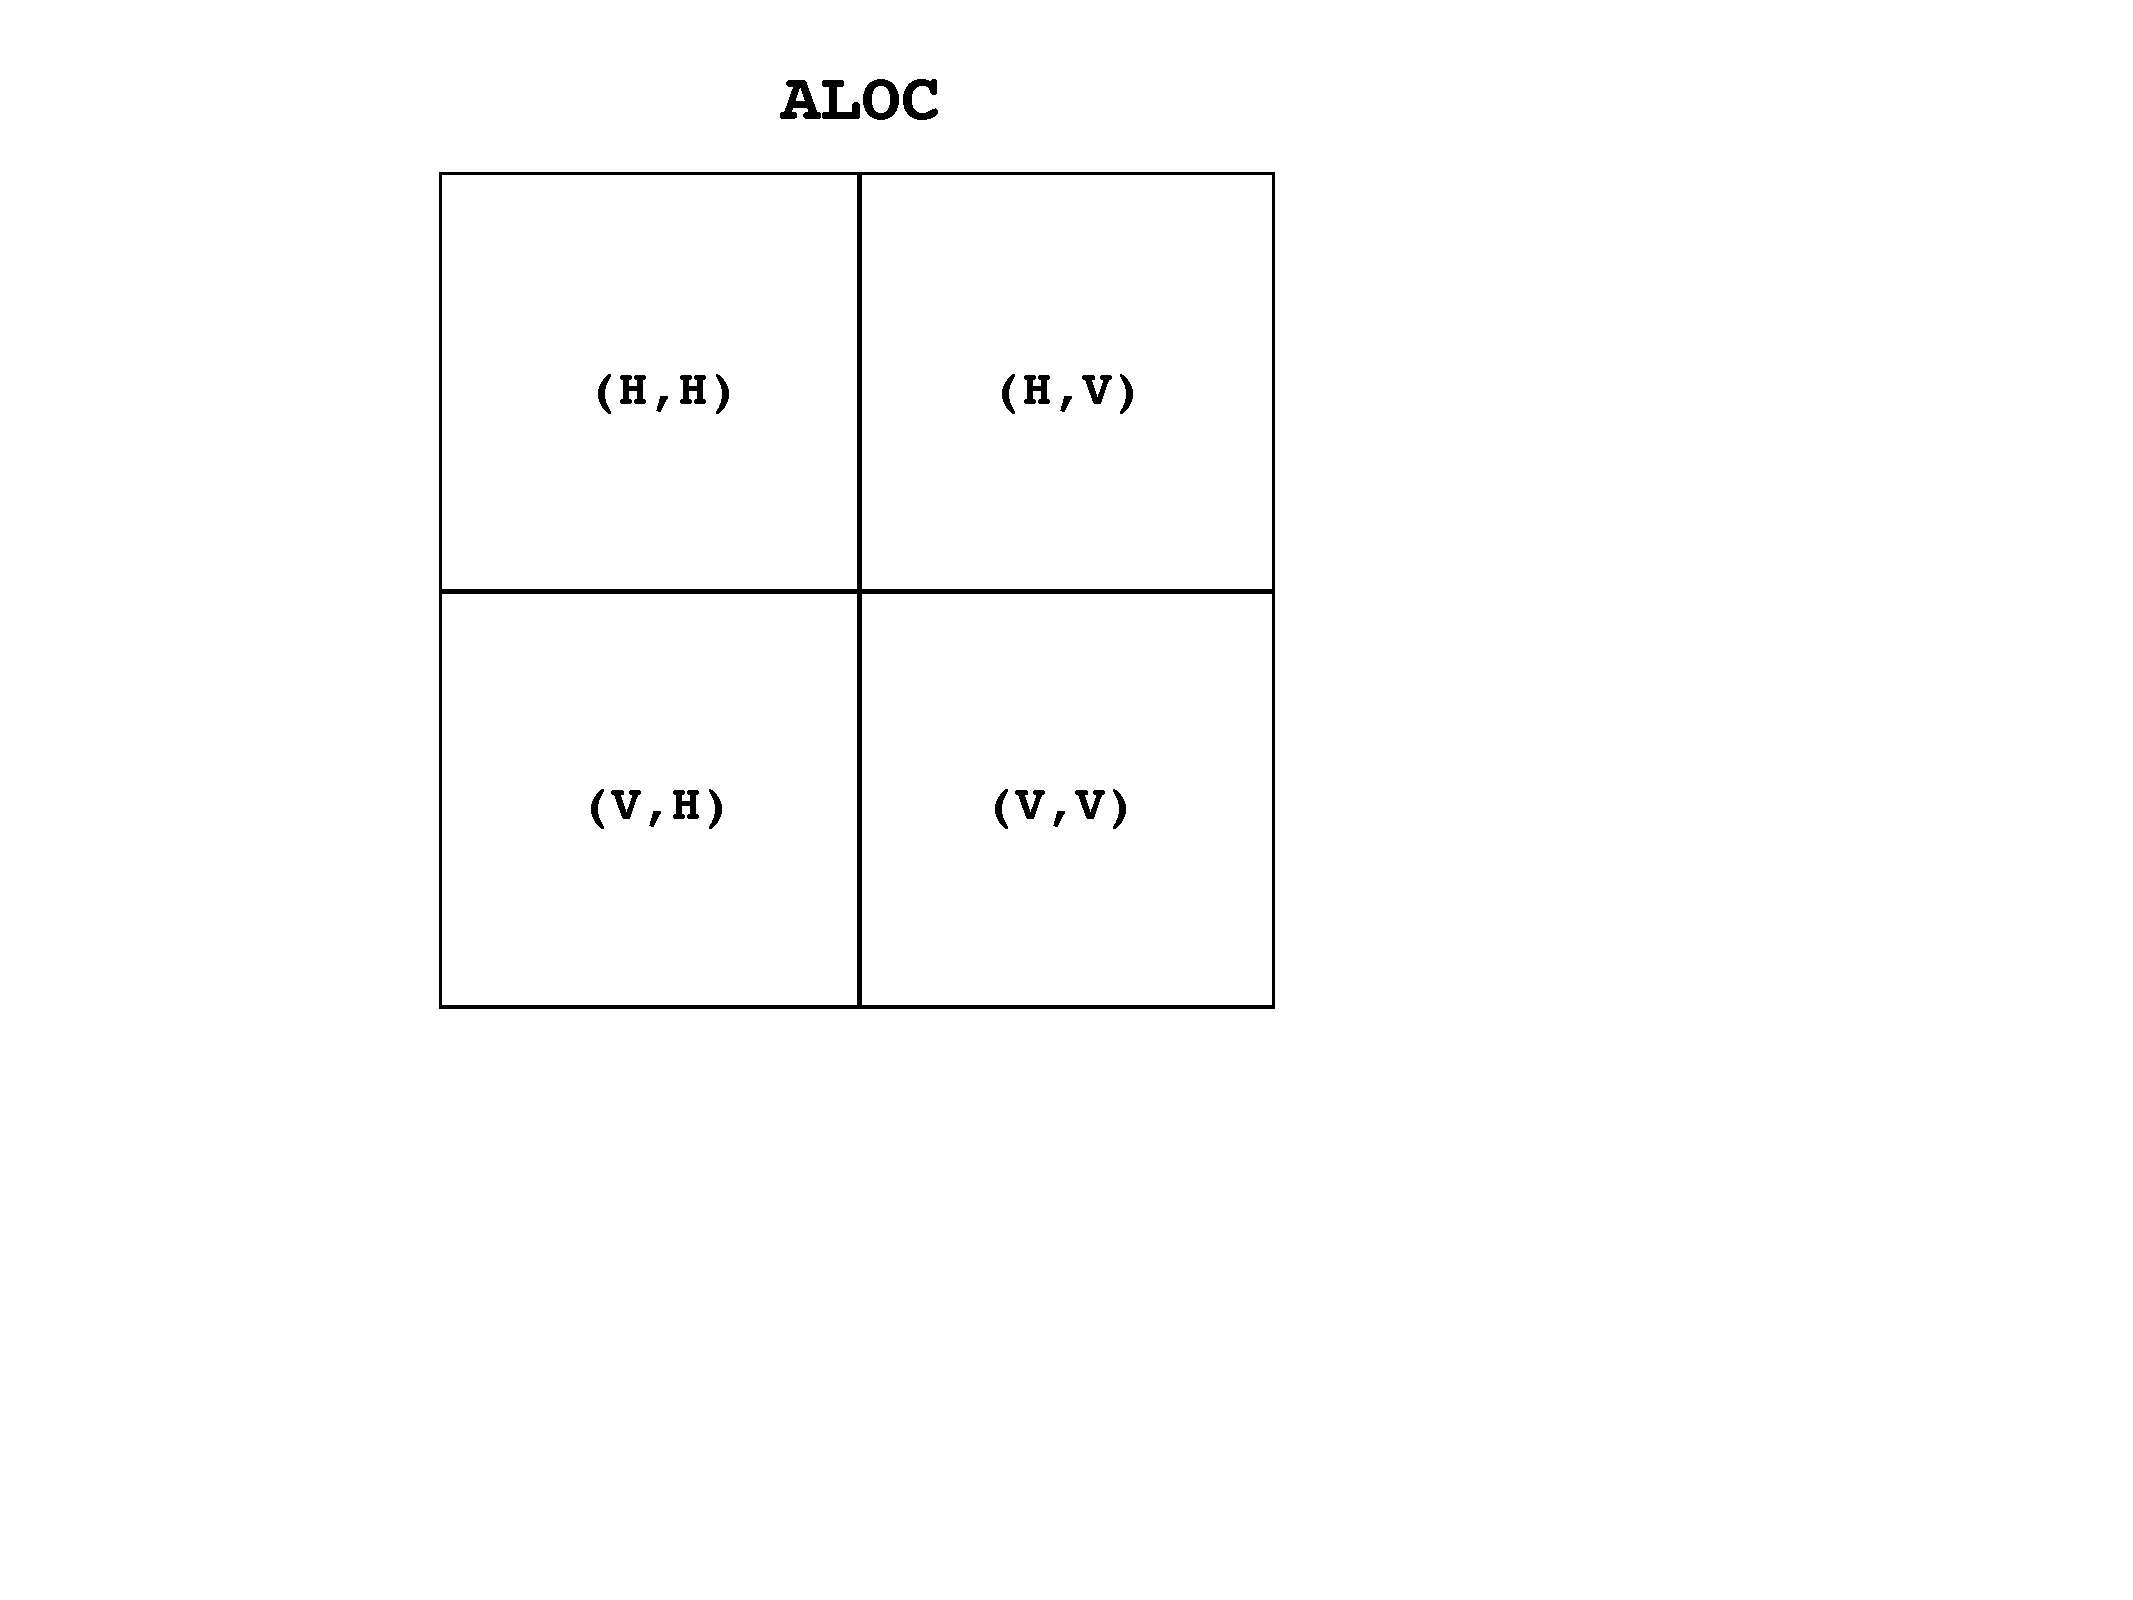
\includegraphics[height=1.8in]{ALOC.pdf}
	\end{subfigure}
	\begin{subfigure}[b]{0.3\textwidth}
		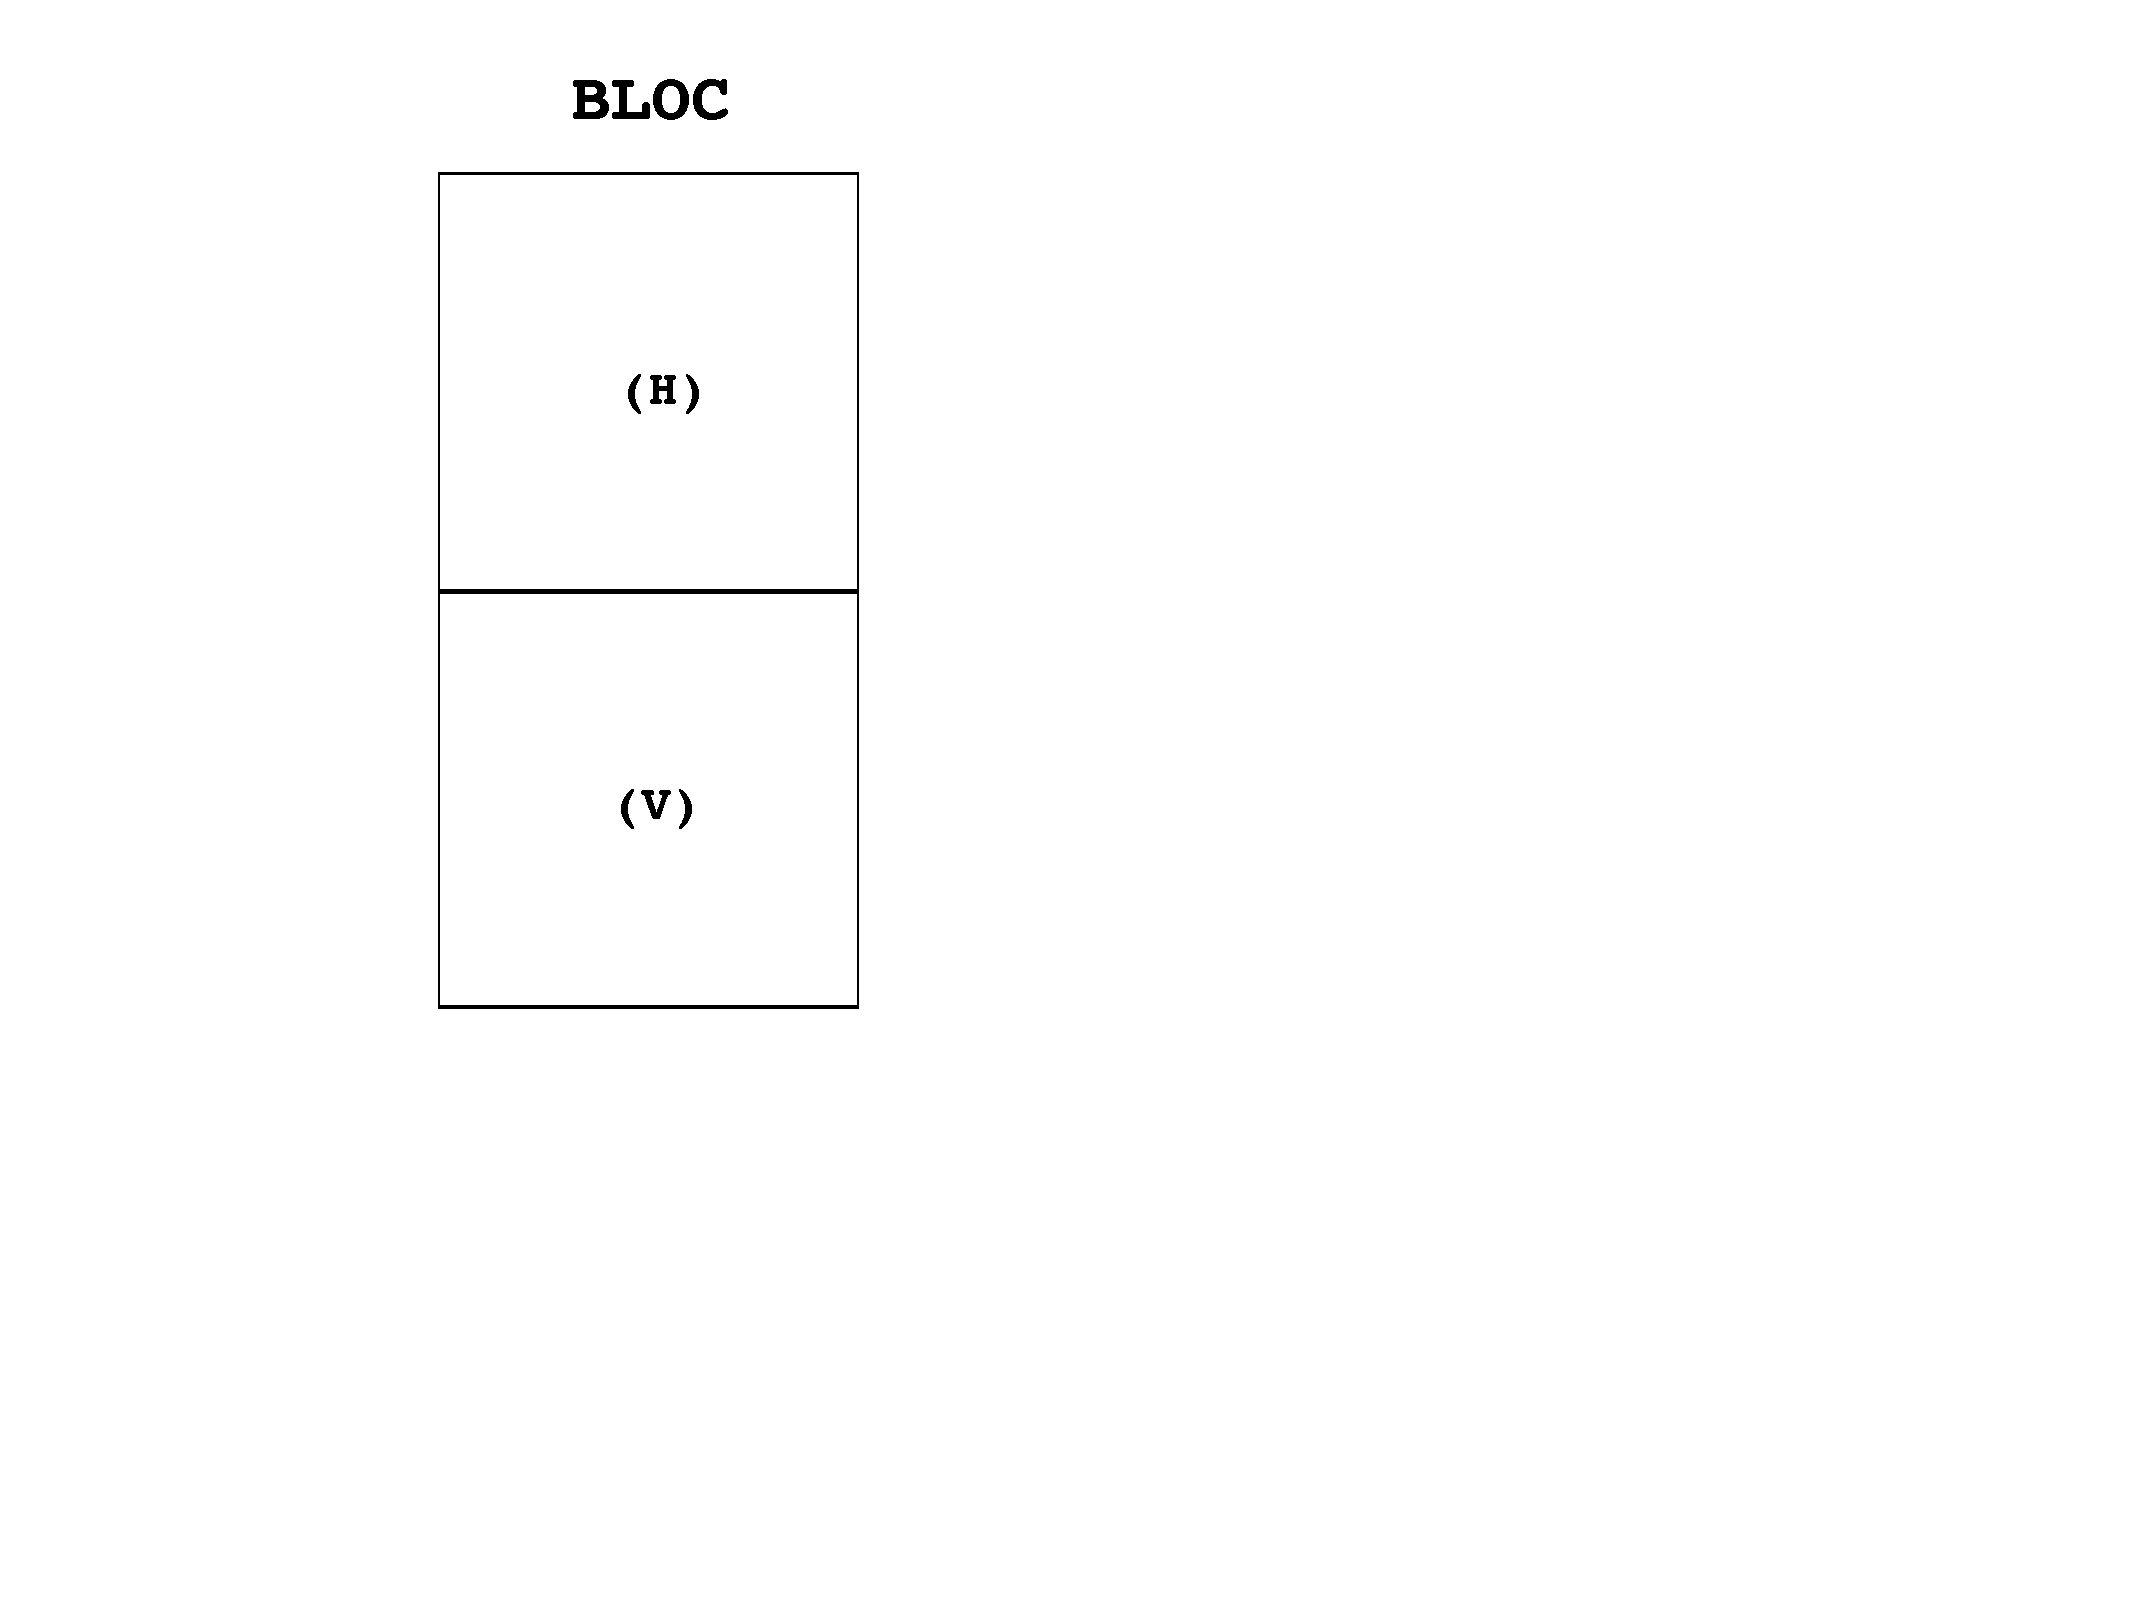
\includegraphics[height=1.8in]{BLOC.pdf}
	\end{subfigure}
	\caption*{Element-local system.}
\end{figure}
\end{minipage}

\vskip 5pt
\begin{minipage}[t]{0.60\textwidth}
Recall the statically condensed system\\[-5pt]
(cf.~Appendix~\ref{chap:dpg}): \vspace{-10pt}
\[
	\left[ \begin{array}{cc}
		\mr{B^* G^{-1} B} & \mr{B^* G^{-1} \hat B} \\
		\mr{\hat B^* G^{-1} B} & \mr{\hat B^* G^{-1} \hat B} \\
	\end{array} \right]
	\left[ \begin{array}{c}
		\mr{u_h} \\
		\mr{\hat u_h} 
	\end{array} \right]
	=
	\left[ \begin{array}{c}
		\mr{B^* G^{-1} l} \\
		\mr{\hat B^* G^{-1} l}
	\end{array} \right]
\]
\end{minipage}
\begin{minipage}[t]{0.39\textwidth}
Auxiliary local variables: \vspace{-10pt}
\begin{itemize}
	\itemsep -8pt
	\item \var{stiff\_HH} $\leftarrow \mr B$
	\item \var{stiff\_HV} $\leftarrow \mr{\hat B}$
	\item \var{bload\_H} $\leftarrow \mr l$
	\item \var{stiff\_ALL} $\leftarrow \left[ \mr{B \, | \, \hat B \, | \, l \, } \right]$
\end{itemize}
\end{minipage}

\vskip 5pt

In the \routine{elem} routine, these steps are implemented as follows:
\begin{enumerate}
	\item{ Preliminary set up:
\begin{lstlisting}[mathescape,caption=\file{POISSON/PRIMAL\_DPG/}\routine{elem}: preliminary set up]
!..allocate auxiliary matrices
   allocate(gramP(NrTest*(NrTest+1)/2))
   allocate(stiff_HH(NrTest,NrdofH))
   allocate(stiff_HV(NrTest,NrdofVi))
   allocate(bload_H(NrTest))

!..determine element type; number of vertices, edges, and faces
   etype = NODES(Mdle)%ntype
   nrv = nvert(etype); nre = nedge(etype); nrf = nface(etype)
   
!..determine order of approximation (element integrals)
   call find_order(Mdle, norder)
!..determine enriched order of approximation (hexa)
   nordP = NODES(Mdle)%order+NORD_ADD*111

!..determine edge and face orientations
   call find_orient(Mdle, norient_edge,norient_face)
!..determine nodes coordinates
   call nodcor(Mdle, xnod)
   
!  ....... element integrals
\end{lstlisting}
	}
	\item{ Element integration:
\begin{lstlisting}[mathescape,caption=\file{POISSON/PRIMAL\_DPG/}\routine{elem}: element integration]
!..use the enriched order to set the quadrature
   INTEGRATION = NORD_ADD ! $\Delta p \in \{1, 2, \ldots \}$
   call set_3D_int_DPG(etype,norder,norient_face, nrint,xiloc,waloc)

!..loop over integration points
   do l=1,nrint
!  ...coordinates and weight of this integration point
      xi(1:3) = xiloc(1:3,l); wa = waloc(l)

!  ...H1 shape functions (for geometry)
      call shape3DH(etype,xi,norder,norient_edge,norient_face, nrdofH,shapH,gradH)
!  ...discontinuous H1 shape functions
      call shape3HH(etype,xi,nordP, nrdof,shapHH,gradHH)

!  ...geometry map
      call geom3D(Mdle,xi,xnod,shapH,gradH,nrdofH, x,dxdxi,dxidx,rjac,iflag)
!  ...integration weight
      weight = rjac*wa
!  ...get the RHS
      call getf(Mdle,x, fval)

!  ...1st loop through enriched H1 test functions
      do k1=1,nrdofHH
!     ...Piola transformation
         v = shapHH(k1)
         dv(1:3) = gradHH(1,k1)*dxidx(1,1:3) + &
                    gradHH(2,k1)*dxidx(2,1:3) + &
                    gradHH(3,k1)*dxidx(3,1:3)
!
!     ...accumulate load: $(f,v)$
         bload_H(k1) = bload_H(k1) + fval*v*weight
!
!     ...loop through H1 trial functions
         do k2=1,nrdofH
!        ...Piola transformation
            dp(1:3) = gradH(1,k2)*dxidx(1,1:3) + &
                       gradH(2,k2)*dxidx(2,1:3) + &
                       gradH(3,k2)*dxidx(3,1:3)
!
!        ...accumulate stiffness: $(\nabla u, \nabla_h v)$
            stiff_HH(k1,k2) = stiff_HH(k1,k2) + weight*(dv(1)*dp(1)+dv(2)*dp(2)+dv(3)*dp(3))
         enddo

!     ...2nd loop through enriched H1 test functions for Gram matrix
         do k2=k1,nrdofHH
!        ...Piola transformation
            q = shapHH(k2)
            dq(1:3) = gradHH(1,k2)*dxidx(1,1:3) + & 
                       gradHH(2,k2)*dxidx(2,1:3) + &
                       gradHH(3,k2)*dxidx(3,1:3)

!        ...determine index in triangular packed format
            k = (k2-1)*k2/2+k1
!
!        ...accumulate Gram with test inner product: $(v,v)_\test := (v,v) + (\nabla_h v, \nabla_h v)$
            aux = q*v + (dq(1)*dv(1) + dq(2)*dv(2) + dq(3)*dv(3))
            gramP(k) = gramP(k) + aux*weight
         enddo; enddo; enddo
\end{lstlisting}
	}
	\item{ Boundary integration:
\begin{lstlisting}[mathescape,caption=\file{POISSON/PRIMAL\_DPG/}\routine{elem}: boundary integration.]
!..determine order of approximation (boundary integrals)
   norderi(1:nre+nrf) = norder(1:nre+nrf)
   norderi(nre+nrf+1) = 111

!..loop through element faces
   do ifc=1,nrf

!  ...sign factor to determine the outward normal unit vector
      nsign = nsign_param(etype,ifc)

!  ...face type ('tria','quad')
      ftype = face_type(etype,ifc)

!  ...face order of approximation
      call face_order(etype,ifc,norder, norderf)

!  ...set 2D quadrature
      INTEGRATION = NORD_ADD ! $\Delta p$
      call set_2D_int_DPG(ftype,norderf,norient_face(ifc), nrint,tloc,wtloc)

!  ...loop through integration points
      do l=1,nrint

!     ...face coordinates
         t(1:2) = tloc(1:2,l)
!     ...face parametrization
         call face_param(etype,ifc,t, xi,dxidt)

!     ...determine discontinuous H1 shape functions
         call shape3HH(etype,xi,nordP, nrdof,shapHH,gradHH)
!     ...determine element H(div) shape functions (for fluxes), interfaces only (no bubbles)
         call shape3DV(etype,xi,norderi,norient_face, nrdof,shapV,divV)

!     ...determine element H1 shape functions (for geometry)
         call shape3DH(etype,xi,norder,norient_edge,norient_face, nrdof,shapH,gradH)
!     ...geometry map
         call bgeom3D(Mdle,xi,xnod,shapH,gradH,nrdofH,dxidt,nsign, &
                        x,dxdxi,dxidx,rjac,dxdt,rn,bjac)
!     ...integration weight
         weight = bjac*wtloc(l)

!     ...loop through enriched H1 test functions
         do k1=1,nrdofHH
            v = shapHH(k1)

!        ...loop through H(div) trial functions
            do k2=1,nrdofVi
!           ...Piola transformation
               s(1:3) = (dxdxi(1:3,1)*shapV(1,k2) + &
                          dxdxi(1:3,2)*shapV(2,k2) + &
                          dxdxi(1:3,3)*shapV(3,k2)) / rjac
!           ...normal component
               sn = s(1)*rn(1)+s(2)*rn(2)+s(3)*rn(3)
!
!           ...accumulate stiffness: $-\lb \sigma \cdot n, v \rb_{\Gamma_h}$
               stiff_HV(k1,k2) = stiff_HV(k1,k2) - sn*v*weight

            enddo; enddo ! end loop through trial / test functions
   enddo; enddo; ! end loop through integration points / faces
\end{lstlisting}
	}
	\item{ Construction of DPG linear system:
\begin{lstlisting}[mathescape,caption=\file{POISSON/PRIMAL\_DPG/}\routine{elem}: constructing DPG linear system.]
!---------------------------------------------------------------------
!  Construction of statically condensed DPG linear system
!---------------------------------------------------------------------

!..create auxiliary matrix for dense linear algebra
   allocate(stiff_ALL(NrTest,NrTrial+1))

!..Total test/trial DOFs of the element
   i = NrTest ; j1 = NrdofH ; j2 = NrdofVi

!..Copy stiffness and load into one matrix: $\text{\var{stiff\_ALL}} \leftarrow [ \mr{B \, | \, \hat B \, | \, l \, } ]$
   stiff_ALL(1:i,1:j1)          = stiff_HH(1:i,1:j1)
   stiff_ALL(1:i,j1+1:j1+j2) = stiff_HV(1:i,1:j2)
   stiff_ALL(1:i,j1+j2+1)       = bload_H(1:i)

   deallocate(stiff_HH,stiff_HV)

!..A. Compute Cholesky factorization of Gram Matrix, $\mr{G=U^T U \, (=LL^T)}$
   call DPPTRF('U',NrTest,gramP,info)
!
!..B. Solve triangular system to obtain $\mr{\tilde B,\ \text{i.e.~solve } (L \tilde B=)\, U^T \tilde B = [B \, | \, l]}$
   call DTPTRS('U','T','N',NrTest,NrTrial+1,gramP,stiff_ALL,NrTest,info)

   allocate(raloc(NrTrial+1,NrTrial+1)); raloc = ZERO

!..C. Matrix multiply: $\mr{B^T G^{-1} B \, (=\tilde B^T \tilde B)}$
   call DSYRK('U','T',NrTrial+1,NrTest,ZONE,stiff_ALL,NrTest,ZERO,raloc,NrTrial+1)

!..D. Fill lower triangular part of Hermitian matrix $\mr{\tilde B^T \tilde B}$
   do i=1,NrTrial
      raloc(i+1:NrTrial+1,i) = raloc(i,i+1:NrTrial+1)
   enddo

!..raloc has now all blocks of the stiffness and load:
!  $r_{\text{aloc}} = \var{ALOC(1,1)} \quad \var{ALOC(1,2)} \quad \var{BLOC(1)}$
!         $\, \var{ALOC(2,1)} \quad \var{ALOC(2,2)} \quad \var{BLOC(2)}$
\end{lstlisting}
	}
\end{enumerate}

\subsection{DPG ultraweak implementation}
\label{sec:poisson-ultraweak}
Broken ultraweak formulation:

\[
\left\{
\begin{array}{llll}
	\left\langle \lambda, \bs \tau \cdot n \right\rangle \in H^{1/2}(\Gamma_h) \times H(div,\Omega_h),\,\left \langle \hat{\sigma}_n,v \right \rangle \in H^{1/2}(\Gamma_h) \times H^1(\Omega_h):  u = u_0 \text{ on } \Gamma \, , \\[5pt]
	(u, \nabla \cdot \bs \tau) + (\bs \sigma, \bs \tau + \nabla v) - \lb \hat{\sigma}_n , v \rb_{\Gamma_h} -  \lb \lambda, \bs \tau \cdot \bs n \rb_{\Gamma_h} 
	= (f,v) \, ,\quad v \in H^1(\Omega_h), \bs \tau \in H(div; \Omega_h) \, .
\end{array}
\right.
\]

Ultraweak implementation of DPG differs from both the Galerkin and the primal DPG in the \routine{elem} routine. The static condenstation of the Riesz represntation of the residual is done at the element level (similar to primal DPG implememtation in~\ref{sec:poisson-primal}). 

The imeplementation is provided in \file{problems/POISSON/ULTRAWEAK\_DPG}.
Compared to the primal DPG, the changes in the \file{physics} file are:

\begin{lstlisting}[caption=\file{POISSON/ULTRAWEAK\_DPG/input/physics} input file.]
1025000              MAXNODS,  nodes anticipated
4                    NR_PHYSA, physics attributes
trace_a contin  1    H1 Variable
trace_b normal  1    H(div) variable
field    discon  1   L2 variable
grad     discon  3   L2 Variable
\end{lstlisting}

In ultraweak formulation, there are four physics unknown--- $u$, $\bs \sigma$, $\hat{\sigma}_n$ and $\lambda$, i.e. \code{\var{NR\_PHYSA}=4}. Compared to the primal DPG formulation, additional $L^2$ and trace unknown $\lambda \in H^{1/2}$ are defined in \file{physics} file; the trace of u given by $\lambda$ must later be sepcified as such by setting \code{\var{PHYSAi(1)}=.true.} along with $\hat{\sigma}_n$ (\code{\var{PHYSAi(2)}=.true.}). The \routine{elem} can be split into three distinct steps:

\begin{minipage}{0.48\textwidth}
\begin{enumerate}
	\itemsep -10pt
	\item Element integration \vspace{-15pt}
	\begin{itemize}
		\itemsep -8pt
		\item Stiffness: $\mr B$
		\item Load: $\mr l$
		\item Gram matrix: $\mr G$
	\end{itemize}
	\item Boundary integration \vspace{-15pt}
	\begin{itemize}
		\itemsep -8pt
		\item Stiffness: $\mr{\hat B_{1,1}, \hat B_{1,2}, \hat B_{2,1}, \hat B_{2,2}}$
	\end{itemize}
	\item Constructing DPG linear system \vspace{-15pt}
	\begin{itemize}
		\itemsep -8pt
		\item Dense linear algebra
		\item {Statically condensed system\\[-5pt] 
		stored in \var{ALOC}, \var{BLOC}}
	\end{itemize}
\end{enumerate}
\end{minipage}%
\begin{minipage}{0.48\textwidth}
\begin{figure}[H]
	\centering
		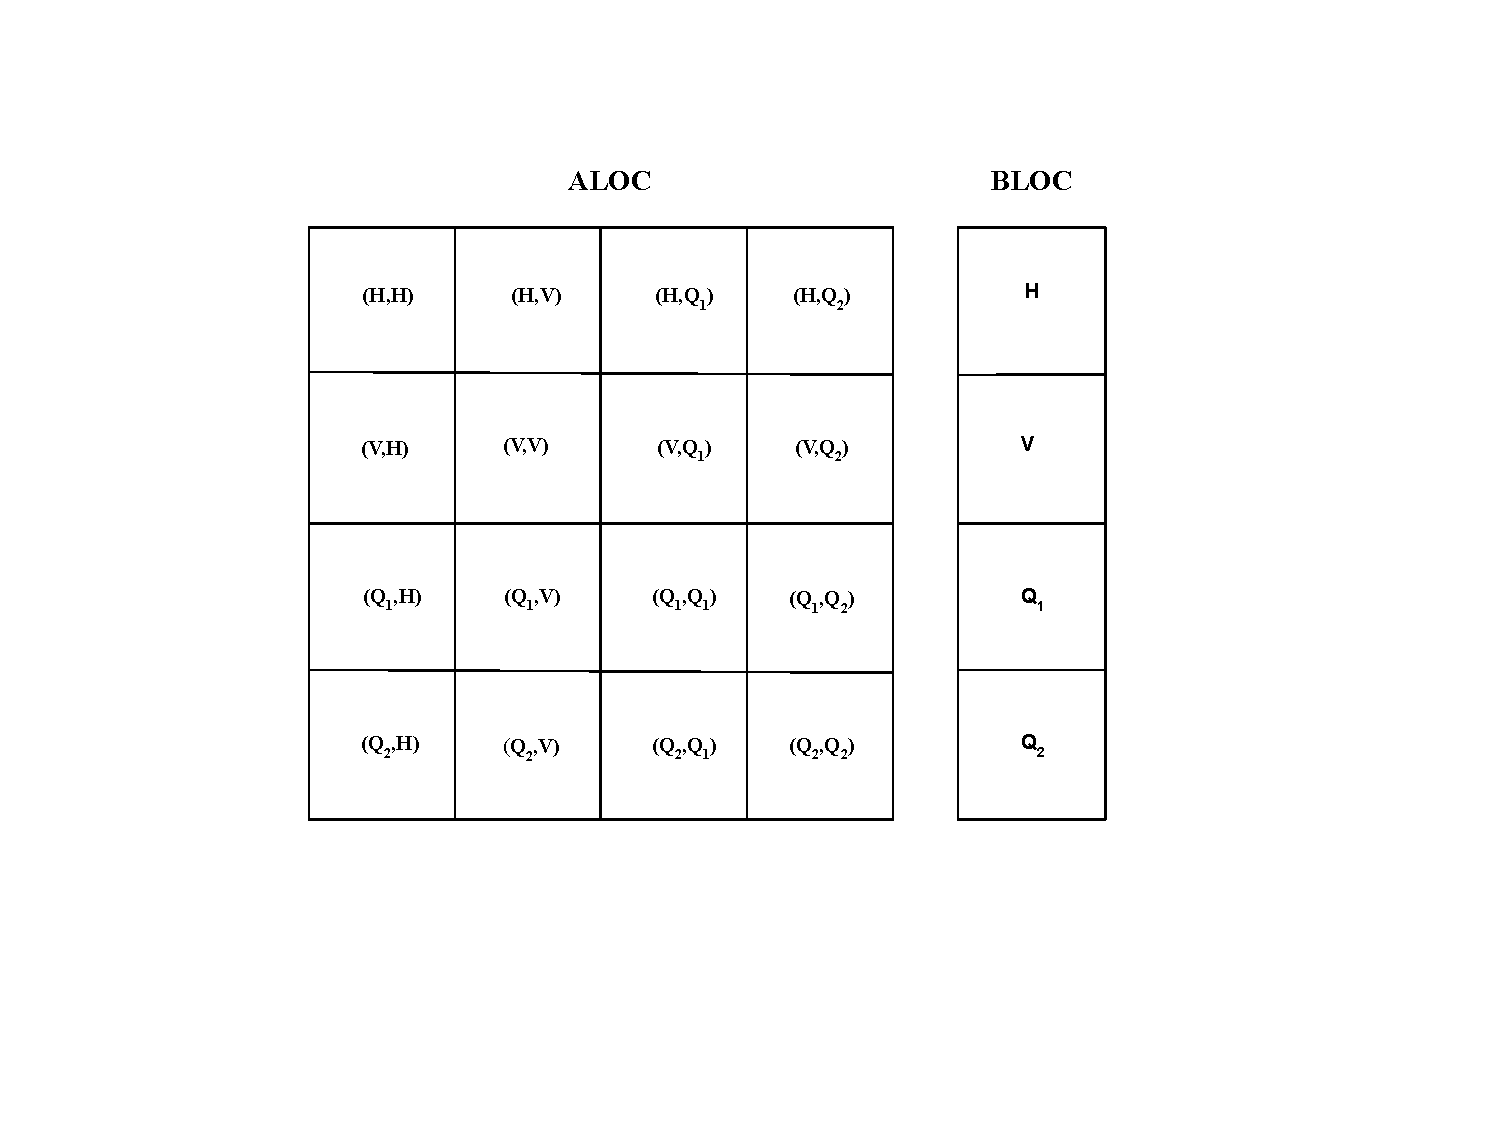
\includegraphics[scale=0.5]{ALOC_UW.pdf}
	\caption*{Element-local system.}
\end{figure}
\end{minipage}

\vskip 5pt
%\begin{minipage}[t]{0.60\textwidth}
%%Recall the statically condensed system\\[-5pt]
%(cf.~Appendix~\ref{chap:dpg}): \vspace{-10pt}
%\[
%  \var{stiff\_ALL}^* G^{-1} \var{stiff\_ALL} = \var{stiff\_ALL}^* G^{-1} \var{bload\_H} 
%\]
%\end{minipage}
\begin{minipage}[t]{\textwidth}
Auxiliary local variables: \vspace{-10pt}
\begin{itemize}
	\itemsep -8pt
	\item \var{stiff\_HH} $\leftarrow \mr{\hat B_{1,1}}$
	\item \var{stiff\_HV} $\leftarrow \mr{\hat B_{1,2}}$
	\item \var{stiff\_HQ1} $\leftarrow \mr{B_{1,3}}$
	\item \var{stiff\_HQ2} $\leftarrow \mr{B_{1,4}}$
	\item \var{stiff\_VH} $\leftarrow \mr {\hat B_{2,1}}$
	\item \var{stiff\_VV} $\leftarrow \mr{\hat B_{2,2}}$
	\item \var{stiff\_VQ1} $\leftarrow \mr{B_{2,3}}$
	\item \var{stiff\_VQ2} $\leftarrow \mr{B_{2,4}}$
	
	\item \var{bload\_H} $\leftarrow \mr {\left[ {l} \, | \, 0\right]}^T$
	\item \vskip 4pt \var{stiff\_ALL} $\leftarrow \left[\begin{array}{c|c|c|c|c}
	\hat B_{1,1} \, | \, & \hat B_{1,2} \, | \, & B_{1,3} \, | \, & B_{1,4} \, | \, & \text{l} \\ \hline
	\hat B_{2,1} \, | \, & \hat B_{2,2} \, | \, & B_{2,3} \, | \, & B_{2,4} \, | \, & 0
	\end{array} \right]$
\end{itemize}
\end{minipage}

The preliminary setup for the ultraweak formulation is simlar to setup of the primal DPG implementation with additional memory allocation for additional unknowns and test functions. The element integration routine for the ultraweak DPG formulation is given by the following code:
\begin{lstlisting}[mathescape,caption=\file{POISSON/ULTRAWEAK\_DPG/}\routine{elem}: element integration]
!..use the enriched order to set the quadrature
   INTEGRATION = NORD_ADD ! $\triangle p \in \{1,2,....\}$
   call set_3D_int_DPG(etype,norder,norient_face, nint,xiloc,waloc)
!
!..loop over integration points
   do l=1,nint
!
!..coordinates and weight of this integration point
      xi(1:3)=xiloc(1:3,l)
      wa=waloc(l)
!
!..H1 shape functions (for geometry)
      call shape3DH(etype,xi,norder,norient_edge,norient_face, nrdof,shapH,gradH)

!..L2 shape functions
      call shape3DQ(etype,xi,norder, nrdof,shapQ)
!
!..discontinuous H1 shape functions
      call shape3HH(etype,xi,nordP, nrdof,shapHH,gradHH)
!..discontinuous H(div) shape functions
      call shape3VV(etype,xi,nordP, nrdof,shapVV,divVV)

!..geometry map
      call geom3D(Mdle,xi,xnod,shapH,gradH,NrdofH, x,dxdxi,dxidx,rjac,iflag)
!
!..integration weight
      weight = rjac*wa
!
!..get the RHS
      call getf(Mdle,x, fval)
!
!..1st loop through enriched H1 test functions
      do k1=1,NrdofHH
!..Piola transformation
         v = shapHH(k1)
         dv(1:3) = gradHH(1,k1)*dxidx(1,1:3) &
                 + gradHH(2,k1)*dxidx(2,1:3) &
                 + gradHH(3,k1)*dxidx(3,1:3)
!
!..accumulate load vector: $\mr{(f,v)}$
         bload_H(k1) = bload_H(k1) + fval*v*weight
!
!..loop through L2 trial functions
         do k2=1,NrdofQ
!
            do ivar = 1,3
               n1 = k1
               n2 = (k2 - 1)*3 + ivar
               sig = ZERO
!..Piola Transform for L2 fields i.e for the $\mr{{ivar}^{th}}$ component of sigma
               sig(ivar) = shapQ(k2)/rjac 
!..acumulate stiffness: $\mr{(\bs \sigma,\nabla v)}$
               stiff_HQ2(n1,n2) = stiff_HQ2(n1,n2) + weight * (sig(1) * dv(1) &
                                                            +sig(2) * dv(2) + sig(3)*dv(3))
            enddo
!
!..end of loop through L2 trial functions
         enddo
!
!..2nd loop through enriched H1 test functions for Gram matrix
         do k2=k1,NrdofHH
!..Piola transformation
            q = shapHH(k2)
            dq(1:3) = gradHH(1,k2)*dxidx(1,1:3) &
                    + gradHH(2,k2)*dxidx(2,1:3) &
                    + gradHH(3,k2)*dxidx(3,1:3)
!
!..determine index in triangular packed format            
            k = nk(k1,k2)
!..accumulate components of Gram matrix correspoding to $\mr{v}$. 
            aux = q*v + (dq(1)*dv(1) + dq(2)*dv(2) + dq(3)*dv(3))
            gramP(k) = gramP(k) + aux*weight
!           
!..end of 2nd loop through enriched H1 test functions
         enddo
!
!..cross terms for  graph norm
         do k2 = 1,NrdofVV
            tau_a(1:3) =     dxdxi(1:3,1) * shapVV(1,k2)      &
                           + dxdxi(1:3,2) * shapVV(2,k2)       &
                           + dxdxi(1:3,3) * shapVV(3,k2)
            
            tau_a(1:3) = tau_a(1:3)/rjac
            k = nk(k1,NrdofHH+k2)
!..accumulate components of Gram matrix correspoding to inner products involving $\mr{v}$ and $\mr{\bs \tau}$. 
            aux = dv(1) * tau_a(1) + dv(2) * tau_a(2) + dv(3) * tau_a(3)
            gramP(k) = gramP(k) + aux * weight
         enddo
!
!..end of 1st loop through enriched H1 test functions
      enddo
!..loop over discontinuous H(div) test functions
      do k1=1,NrdofVV
!..Piola transformation
         divtau_a = divVV(k1)/rjac
         tau_a(1:3) =     dxdxi(1:3,1) * shapVV(1,k1)      &
                        + dxdxi(1:3,2) * shapVV(2,k1)       &
                        + dxdxi(1:3,3) * shapVV(3,k1)
!
         tau_a(1:3) = tau_a(1:3)/rjac   
!         
         do k2=1,NrdofQ
!..Piola transformation
            u = shapQ(k2)/rjac
!..accumulate stiffness: $\mr{(u,\nabla \cdot \bs \tau)}$
            stiff_VQ1(k1,k2) = stiff_VQ1(k1,k2) + weight*(u * divtau_a)
!
            do ivar = 1,3
               sig = ZERO
               sig(ivar) = shapQ(k2)/rjac  !Piola transform for the $\mr{{ivar}^{th}}$ component
               n1 = k1
               n2 = (k2 - 1)*3 + ivar
!..accumulate stiffness: $\mr{(\bs \sigma,\bs \tau)}$
               stiff_VQ2(n1,n2) = stiff_VQ2(n1,n2) + weight*(tau_a(1)*sig(1) + tau_a(2) * sig(2) &
                                                          + tau_a(3)*sig(3))
!
            enddo
         enddo
!
!..Gram matrix contribution for H(div) inner product
         do k2=k1,NrdofVV
!..Piola transformation
            divtau_b = divVV(k2)/rjac
            tau_b(1:3) =     dxdxi(1:3,1) * shapVV(1,k2)      &
                           + dxdxi(1:3,2) * shapVV(2,k2)       &
                           + dxdxi(1:3,3) * shapVV(3,k2)
!   
            tau_b(1:3) = tau_b(1:3)/rjac
!
            k = nk(k1 + NrdofHH,k2 + NrdofHH)
            aux = divtau_a * divtau_b + 2.d0 * (tau_a(1)*tau_b(1) + tau_a(2)*tau_b(2) + tau_a(3)*tau_b(3))
            gramP(k) = gramP(k) +  weight * aux
!
         enddo   
!..end of loop on H(div) test functions
      enddo
!
!..end of loop through integration points
   enddo
\end{lstlisting}

Next, we provide the code peforming the boundary integration:
\begin{lstlisting}[mathescape,caption=\file{POISSON/ULTRAWEAK\_DPG/}\routine{elem}: boundary integration]
!
!---------------------------------------------------------------------
!    B O U N D A R Y    I N T E G R A L S                            |
!---------------------------------------------------------------------
! 
!
!..loop through element faces
   do ifc=1,nrf
!
!..sign factor to determine the outward normal unit vector
      nsign = nsign_param(etype,ifc)
!
!..face type
      ftype = face_type(etype,ifc)
!
!..face order of approximation
      call face_order(etype,ifc,norder, norderf)
!
!..set 2D quadrature
      INTEGRATION = NORD_ADD
      call set_2D_int_DPG(ftype,norderf,norient_face(ifc), nint,tloc,wtloc)
      INTEGRATION = 0
!
!..loop through integration points
      do l=1,nint
!
!..face coordinates
         t(1:2) = tloc(1:2,l)
!
!..face parametrization
         call face_param(etype,ifc,t, xi,dxidt)
!
!..determine discontinuous H1 shape functions
         call shape3HH(etype,xi,nordP, nrdof,shapHH,gradHH)
!..discontinuous H(div) shape functions
         call shape3VV(etype,xi,nordP, nrdof,shapVV,divVV)
!
!..determine element H1 shape functions (for geometry)
         call shape3DH(etype,xi,norder,norient_edge,norient_face, &
                       nrdof,shapH,gradH)
!
!..determine H(div) shape functions (for fluxes) on face
         call shape3DV(etype,xi,norderi,norient_face, &
                       nrdof,shapV,divV)

!..geometry map
         call bgeom3D(Mdle,xi,xnod,shapH,gradH,NrdofH,dxidt,nsign, &
                  x,dxdxi,dxidx,rjac,dxdt,rn,bjac)
!..integration weight
         weight = bjac*wtloc(l)
!
!..loop through enriched H1 test functions
         do k1=1,NrdofHH
            v = shapHH(k1)
!
!..loop through H(div) trial functions on face
            do k2=1,NrdofVi_b
!..Piola transformation
               s(1:3) = dxdxi(1:3,1)*shapV(1,k2) &
                        + dxdxi(1:3,2)*shapV(2,k2) &
                        + dxdxi(1:3,3)*shapV(3,k2)
               s(1:3) = s(1:3)/rjac
!..normal component
               sn = s(1)*rn(1)+s(2)*rn(2)+s(3)*rn(3)
!
!..accumulate stiffness: -$\mr{\left\langle \hat{\sigma}_n,v \right\rangle}$
               stiff_HV(k1,k2) = stiff_HV(k1,k2) - sn*v*weight
!..end of loop through H(div) trial functions on face
            enddo
!..end of loop through enriched H1 test functions
         enddo

!..loop through enriched H(div) test functions
         do k1=1,NrdofVV
!..Piola Transform
            tau_a(1:3) =     dxdxi(1:3,1) * shapVV(1,k1)      &
                           + dxdxi(1:3,2) * shapVV(2,k1)       &
                           + dxdxi(1:3,3) * shapVV(3,k1)
!
            tau_a(1:3) = tau_a(1:3)/rjac
            tn = tau_a(1)*rn(1) + tau_a(2)*rn(2) + tau_a(3)*rn(3)
            do k2=1,NrdofVi_a
               lambda = shapH(k2)
!
!..accumulate stiffness: $\mr{-\left\langle \lambda,\bs \tau \cdot \bs n \right\rangle}$
               stiff_VH(k1,k2) = stiff_VH(k1,k2) - weight * tn * lambda
!..end of loop through H1 trial functions
            enddo
!..end of loop through enriched H(div) test functions
         enddo   
!
!..end of loop through integration points
      enddo
!..end of loop through element faces
   enddo

\end{lstlisting}
Finally, the code performing the construction of the DPG linear system.
\begin{lstlisting}[mathescape,caption=\file{POISSON/ULTRAWEAK\_DPG/}\routine{elem}: constructing DPG linear system.]

!---------------------------------------------------------------------
!  Construction of DPG system
!---------------------------------------------------------------------
!
   allocate(stiff_ALL(NrTest,NrTrial+1))
   stiff_ALL = ZERO
!
!  Total test/trial DOFs of the element
   i1 = NrdofHH; i2 = NrdofVV; j1 = NrdofVi_a; j2 = NrdofVi_b; j3 = NrdofU; j4 = NrdofS
!
!..Copy stiffness and load into one matrix
!
   stiff_ALL(1:i1,1:j1) = stiff_HH
   stiff_ALL(1:i1,j1+1:j1+j2) = stiff_HV
   stiff_ALL(1:i1,j1+j2+1:j1+j2+j3) = stiff_HQ1
   stiff_ALL(1:i1,j1+j2+j3+1:j1+j2+j3+j4) = stiff_HQ2
!
   stiff_ALL(i1+1:i1+i2,1:j1) = stiff_VH
   stiff_ALL(i1+1:i1+i2,j1+1:j1+j2) = stiff_VV
   stiff_ALL(i1+1:i1+i2,j1+j2+1:j1+j2+j3) = stiff_VQ1
   stiff_ALL(i1+1:i1+i2,j1+j2+j3+1:j1+j2+j3+j4) = stiff_VQ2
!
   stiff_ALL(1:i1+i2,j1+j2+j3+j4+1) = bload_H
!
   deallocate(stiff_HQ1,stiff_HQ2,stiff_HH,stiff_HV)
   deallocate(stiff_VQ1,stiff_VQ2,stiff_VH,stiff_VV)
!
!..A. Compute Cholesky factorization of Gram Matrix, $\mr{G=U^T U (=LL^T)}$
   call DPPTRF('U',NrTest,gramP,info)
   if (info.ne.0) then
      write(*,*) 'elem_heat: DPPTRF: Mdle,info = ',Mdle,info,'. stop.'
      stop
   endif
!
!..B. Solve triangular system to obtain $\mr{\tilde{B}}$, $\mr{(LX=) U^T X = [B|l]}$
   call DTPTRS('U','T','N',NrTest,NrTrial+1,gramP,stiff_ALL,NrTest,info)
   if (info.ne.0) then
      write(*,*) 'elem_heat: DTPTRS: Mdle,info = ',Mdle,info,'. stop.'
      stop
   endif
!
   allocate(raloc(NrTrial+1,NrTrial+1)); raloc = ZERO

!..C. Matrix multiply: $\mr{B^T G^{-1} B (=\tilde{B}^T \tilde{B})}$
   call DSYRK('U','T',NrTrial+1,NrTest,ZONE,stiff_ALL,NrTest,ZERO,raloc,NrTrial+1)
!
   deallocate(stiff_ALL)
!
!..D. Fill lower triangular part of Hermitian matrix using the upper triangular matrix $\mr{\tilde B^T \tilde B}$
   do i=1,NrTrial
      raloc(i+1:NrTrial+1,i) = raloc(i,i+1:NrTrial+1)
   enddo
   
!..raloc has now all blocks of the stiffness and load:
!  $r_{\text{aloc}} =   \var{ALOC(1,1)} \quad \var{ALOC(1,2)}  \var{ALOC(1,3)} \quad \var{ALOC(1,4)} \quad\var{BLOC(1)}$
!         $\, \var{ALOC(2,1)} \quad \var{ALOC(2,2)}  \var{ALOC(2,3)} \quad \var{ALOC(2,4)} \quad \var{BLOC(2)}$
!         $\, \var{ALOC(3,1)} \quad \var{ALOC(3,2)}  \var{ALOC(3,3)} \quad \var{ALOC(3,4)} \quad \var{BLOC(3)}$
!         $\, \var{ALOC(4,1)} \quad \var{ALOC(4,2)}  \var{ALOC(4,3)} \quad \var{ALOC(4,4)} \quad \var{BLOC(4)}$
\end{lstlisting}

